\section{Implementazione}

\subsection{L'interfaccia}

L'interfaccia utente del sistema è stata rivisitata ed adattata alle nuove esigenze. 

\subsubsection{Pagina di creazione del groundtruth}

\begin{figure*}
\begin{center}
\centering
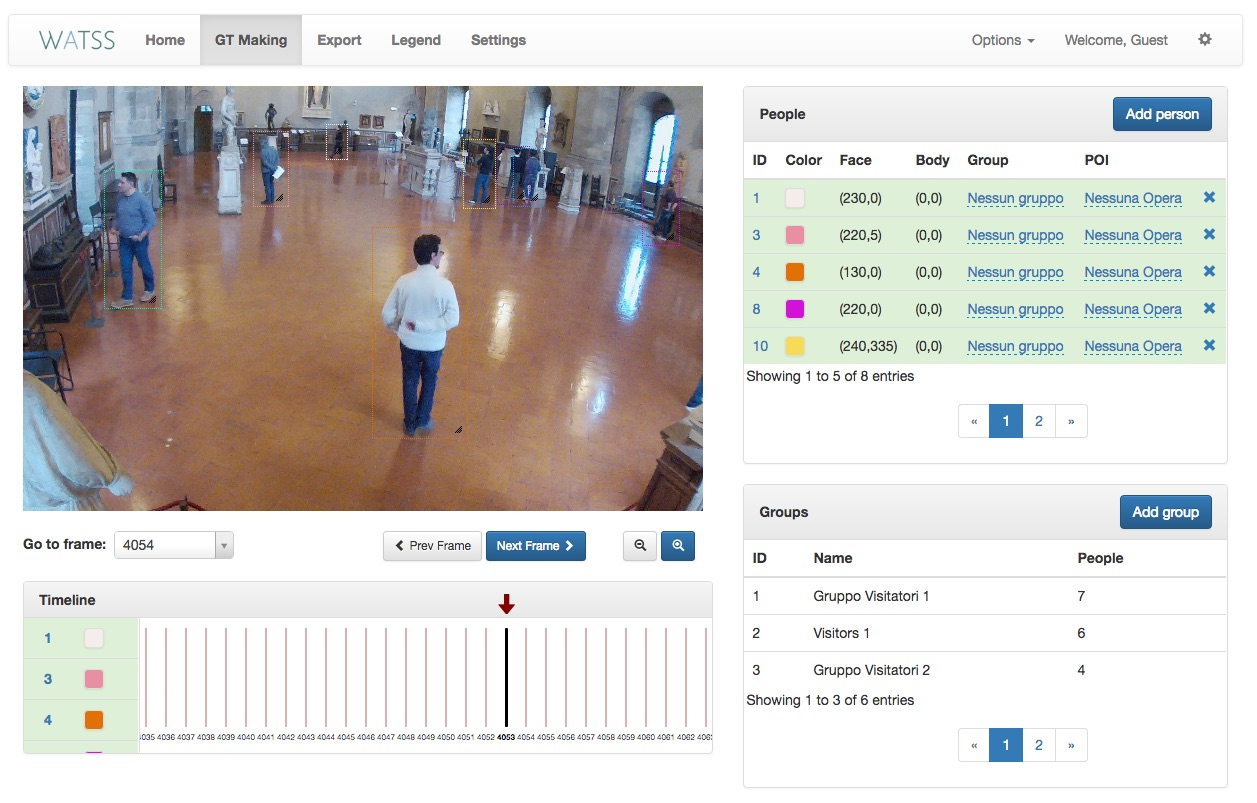
\includegraphics[width=1\linewidth]{images/watss-gui.jpg}
  \label{fig:watss-gui}
  \caption{Interfaccia utente del tool WATSS}
\end{center}
\end{figure*}

La parte principale è costituita dal frame video su cui andremo ad aggiungere annotazioni e visualizzare quelle già esistenti.
I due pannelli laterali per le persone e gruppi presenti nella scena sono stati organizzati in modo tale da consentirne una rapida navigazione ed uso. Come nella precedente versione dell'interfaccia, il pannello \emph{People} mostra la lista delle annotazioni presenti nel frame visualizzato, ordinate in base all'identificativo delle persone. Per ciascuna persona viene mostrato il \emph{gaze }del corpo e della faccia, il \emph{gruppo di appartenenza} ed il \emph{punto di interesse} presso cui si trovano. 

\paragraph{Inserimento di una annotazione}

Tramite il pulsante \emph{Add person} presente nel pannello delle annotazioni è possibile aggiungere una nuova annotazione al frame. 

\begin{figure}[h]
\centering
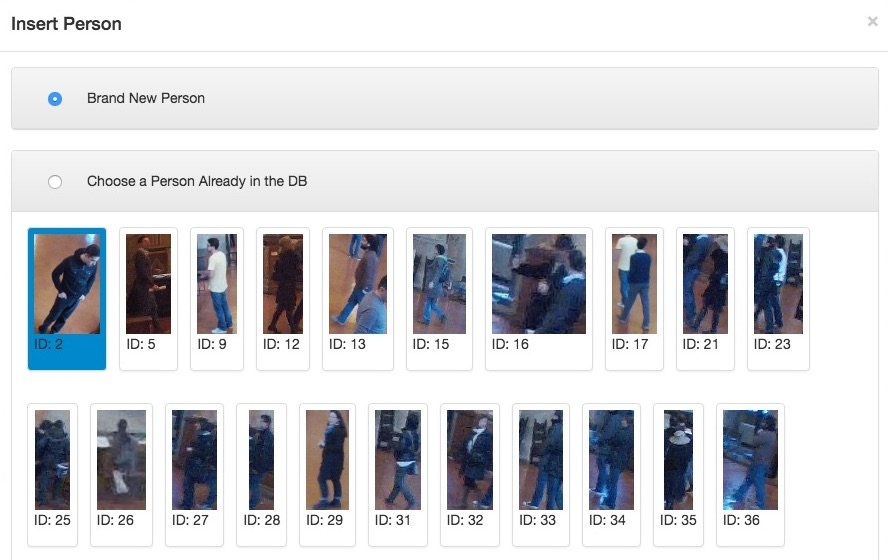
\includegraphics[width=0.8\linewidth]{images/add-person.jpg}
  \caption{Aggiunta di una nuova annotazione}
  \label{fig:addperson}
\end{figure}

Come mostrato in Figura \ref{fig:addperson}, in fase di creazione è possibile indicare se si vuole aggiungere un'annotazione rappresentante una nuova identità ancora non presente nel database oppure se si vuole aggiungere una nuova istanza di un'identità già presente e di cui viene mostrato un \emph{avatar}.

Una volta selezionata l'opzione desiderata, la fase di creazione è diversa in base all'attivazione della \emph{geometria della scena} o meno. Per l'attivazione e la disattivazione della geometria è sufficiente spuntare l'opzione presente nel menù \emph{Options} della barra principale di navigazione.

In caso di geometria della scena \emph{disattivata} la nuova annotazione verrà creata con la tecnica \emph{click and drag}: l'utente clicca nel frame nel punto in cui vuole iniziare la sua selezione e tiene premuto spostando il mouse finchè la bounding box visualizzata non è della dimensione desiderata. A quel punto, rilasciando il click, la bounding box verrà inserita nella scena.

Se invece è attiva la geometria, questa verrà sfruttata per stimare l'altezza di una persona presente nella scena in base alla sua posizione nella stessa. La bounding box verrà automaticamente attaccata al puntatore del mouse e, muovendosi nella scena, sarà ridimensionata in base alla sua posizione. Una volta scelta la posizione, per effettuare l'inserimento sarà sufficiente effettuare un click nel punto desiderato. 

In entrambi i casi, la procedura di inserimento può essere interrotta premendo il tasto \emph{ESC}.

\paragraph{Modifica di una annotazione}

E' stata inoltre migliorata la fase di modifica delle annotazioni presenti. Le bounding box sono ora trascinabili e ridimensionabili mediante il mouse. 

Sia in fase di creazione che di modifica è ora possibile effettuare uno zoom del frame così da poter raffinare delle annotazioni. Questo si è reso necessario soprattutto per quanto riguarda oggetti e persone molto piccoli nella scena. 

Selezionando una bounding box è infine possibile ridimensionarla semplicemente mediante la rotellina del mouse, consentendo una rapida scalatura del rettangolo definito.

\paragraph{La timeline}

La timeline è stata aggiunta all'interfaccia immediatamente sotto il frame. La timeline è così composta:
\begin{itemize}
\item \emph{Elenco dei frames}: vengono visualizzati in ordine crescente in orizzontale. Viene visualizzato un sottoinsieme di frame adiacenti a quello corrente, evidenziato con un cursore a forma di freccia. Per ciascun frame viene indicata la presenza o meno di annotazioni (colore rosso) ed il numero.
\item \emph{Elenco delle annotazioni}: nel pannello laterale sinistro viene mostrato l'elenco delle annotazioni presenti nel frame corrente.
\end{itemize}

\begin{figure}[h]
\centering
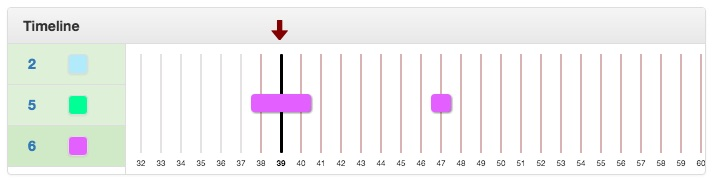
\includegraphics[width=1\linewidth]{images/timeline.jpg}
  \caption{La \emph{timeline}}
  \label{fig:timeline}
\end{figure}

E' possibile navigare tra i frame selezionandone uno dall'elenco e scorrerli mediante il trackpad o la rotellina del mouse.

Selezionando una persona nell'elenco viene mostrata la sua presenza nei frame della timeline mediante una barra orizzontale apposta sopra i frame in cui è presente la stessa persona. 

A partire dalla barra visualizzata è possibile iniziare il processo di generazione dei \emph{proposals} per i frame successivi. Per fare questo è sufficiente trascinare l'estremo destro  della barra fino al frame entro il quale si vuole generare la predizione. Un esempio di generazione di proposals è mostrato in Figura \ref{fig:proposals}.

\begin{figure}[h]
\centering
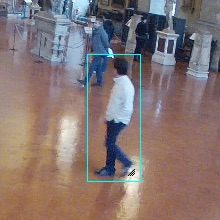
\includegraphics[width=.12\textwidth]{images/proposals/1.jpg}\quad
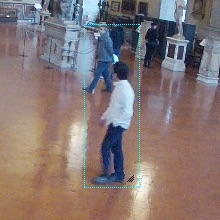
\includegraphics[width=.12\textwidth]{images/proposals/2.jpg}\quad
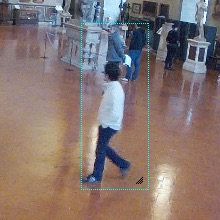
\includegraphics[width=.12\textwidth]{images/proposals/3.jpg}
\medskip
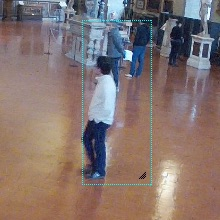
\includegraphics[width=.12\textwidth]{images/proposals/4.jpg}\quad
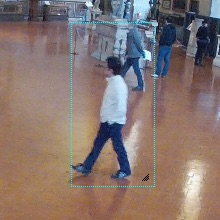
\includegraphics[width=.12\textwidth]{images/proposals/5.jpg}\quad
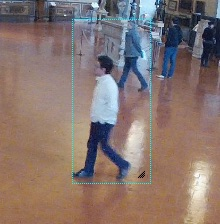
\includegraphics[width=.12\textwidth]{images/proposals/6.jpg}
\caption{Generazione di \emph{proposal} a partire da un'annotazione iniziale}
\label{fig:proposals}
\end{figure}


\subsubsection{Esportazione dei dati}

La pagina di esportazione dei dati è stata ridisegnata al fine di consentire maggiori funzionalità. Nella precedente versione era possibile esportare un'unica tabella contenente le annotazioni presenti nei frames. 

Le funzioni di esportazione si suddividono ora in annotazioni e database: tramite il pannello \emph{Annotations} è possibile selezionare i campi delle annotazioni desiderati e quali frame si vogliono estrarre, mentre tramite il pannello \emph{Database} è possibile esportare la base dati (o solamente lo schema o la combinazione di schema e dati).

\subsubsection{Configurazioni}

Rispetto alla precedente versione, è stata creata una pagina di configurazione del sistema, al fine di rendere lo possibile l'interazione con gli elementi del database direttamente dall'interfaccia.

\begin{figure}[h]
\centering
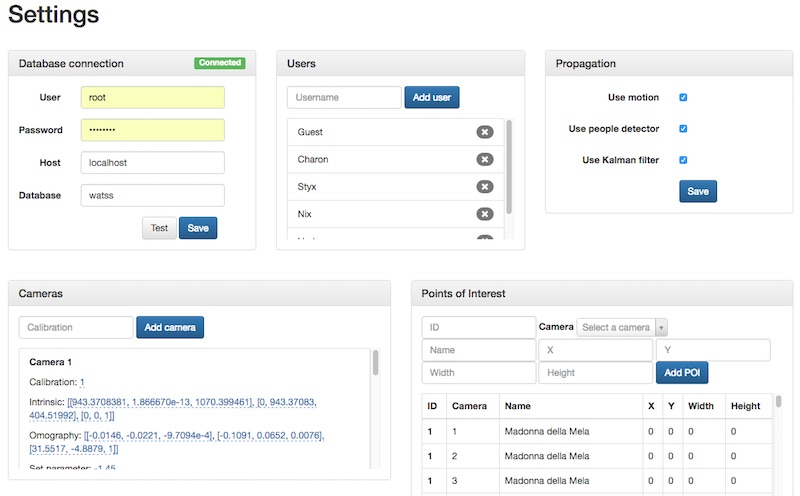
\includegraphics[width=.8\linewidth]{images/settings.jpg}
  \caption{La pagina di configurazione}
  \label{fig:settings}
\end{figure}

Nella pagina di configurazione è possibile:
\begin{itemize}
\item Configurare la \emph{connessione al database}
\item Inserire e rimuovere gli \emph{utenti} che hanno accesso al sistema
\item Aggiungere, rimuovere e impostare la \emph{calibrazione} delle \emph{camere}
\item Aggiungere e rimuovere i \emph{punti di interesse}
\item Selezionare le tecniche usate nella generazione dei \emph{proposals}
\end{itemize} 

Per accedere alla pagina di configurazione è necessario aver preventivamente effettuato l'accesso al sistema.

\subsubsection{Pagina di installazione}

Per agevolare le operazioni di installazione è stata infine creata una pagina dedicata a questo scopo che guida nella procedura tramite interfaccia grafica. 

La procedura di installazione viene descritta in seguito nella Sezione.

\subsection{Tecniche utilizzate}

Vengono ora presentate le tecniche e la teoria alla base rispettivamente della generazione dei \emph{proposals} in fase di annotazione e della geometria della scena, usata nella creazione delle bounding box.

\subsubsection{Generazione dei proposals}

Il problema della generazione di \emph{proposals} per frames successivi a quello/i annotato/i è affrontato mediante una combinazione di più tecniche per la stima del movimento di un oggetto nella scena, nel nostro caso di una persona.

Per questo scopo sono utilizzati:
\begin{itemize}
\item \emph{Motion detection}: rilevazione del movimento mediante tecniche di rimozione dello sfondo di scena.
\item \emph{Pedestrian detector}: un detector di persone basato su \emph{HOG features}.
\item \emph{Filtro di Kalman}: per la stima del moto data una serie di osservazioni passate.
\end{itemize}

Lo script di predizione prende in ingresso un insieme di frame con le rispettive annotazioni di una singola persona e l'insieme di frame su cui si vuole generare un \emph{proposal}. A partire dalle immagini date in ingresso, restituisce un insieme di bounding box rappresentanti la posizione della persona nei frames desiderati. L'implementazione dello script è stata scritta in Python con la libreria OpenCV.

\paragraph{Motion detection}

La tecnica di \emph{motion detection} utilizzata pone le sue basi su quella di \emph{background substraction (BS)}. Dato un generico frame, rimuovendo lo sfondo della scena ottengo una \emph{foreground mask}, ovvero un'immagine binaria contenente i pixel in corrispondenza degli oggetti che si muovono nella scena.

Le tecniche di BS calcolano la \emph{foreground mask} sottraendo al frame corrente il \emph{background model}, addestrato a partire da una serie di frame \emph{statici} forniti in precedenza. La tecnica di BS utilizzata nel progetto è basata sulle \emph{Mixture of Gaussians (MoG)}, direttamente implementate nella libreria OpenCV.

Il metodo MoG opera modellando ciascun pixel come una \emph{mixture of Gaussians} e usa un'approssimazione per aggiornare il modello in linea. I pixel che non rispettano questa approssimazione, o non \emph{fittano} il modello così generato, sono chiamati pixel di \emph{foreground}.

\begin{figure}[h]
\centering
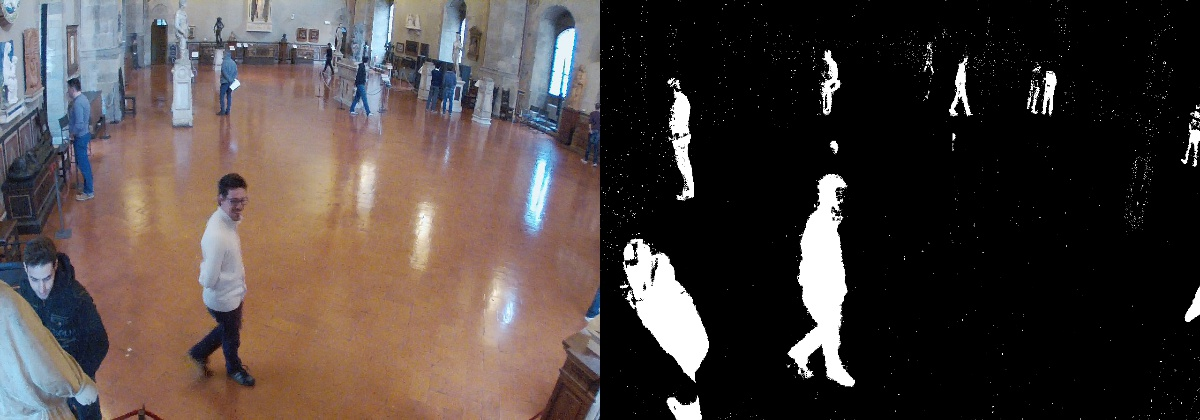
\includegraphics[width=.9\linewidth]{images/frame_mog.jpg}
  \caption{Un esempio di applicazione della tecnica di BS ad un frame}
  \label{fig:mog}
\end{figure}

Il \emph{background model} viene inizialmente addestrato utilizzando 40 frames presi casualmente da tutta la sequenza, così da garantire una varianza più alta possibile.

L'immagine di foreground ottenuta viene processata mediante operazioni morfologiche, apertura e dilatazione, per andare a rimuovere le regioni molto piccole ed unire le regioni molto vicine tra loro. A questo punto vengono estratti i \emph{contorni} delle regioni rimanenti definendo per ciascuna di esse una bounding box che le contiene. Le bounding box inferiori ad un una certa area prefissata (impostata a 500 pixels) vengono scartate).

\paragraph{Pedestrian detection}

Il \emph{pedestrian detector} utilizzato si basa sull'approccio combinato di HOG e SVM. HOG, \emph{Histogram of Oriented Gradients}, è un descrittore globale basato su istogrammi che misurano le orientazioni ed i moduli dei grandienti in una regione dell'immagine.

Il calcolo delle feature HOG si effettua in più passaggi:
\begin{itemize}
\item Calcola gli istogrammi in una parte dell'immagine, una \emph{detection window} tipicamente   $64 \times 128 $ pixels.
\item Crea blocchi di pixel $8 \times 8 $ e calcola gli istorgrammi normalizzati.
\item Concatena gli istogrammi ottenuti.
\end{itemize}

In Figura \ref{fig:detections} vengono mostrate le \emph{detections} dei due metodi distinti.

\begin{figure}[h]
\centering
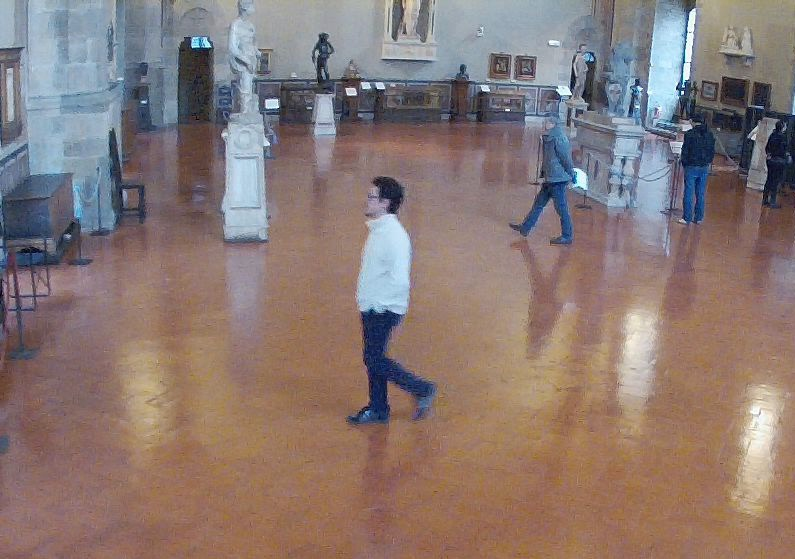
\includegraphics[width=.2\textwidth]{images/original.jpg}\quad
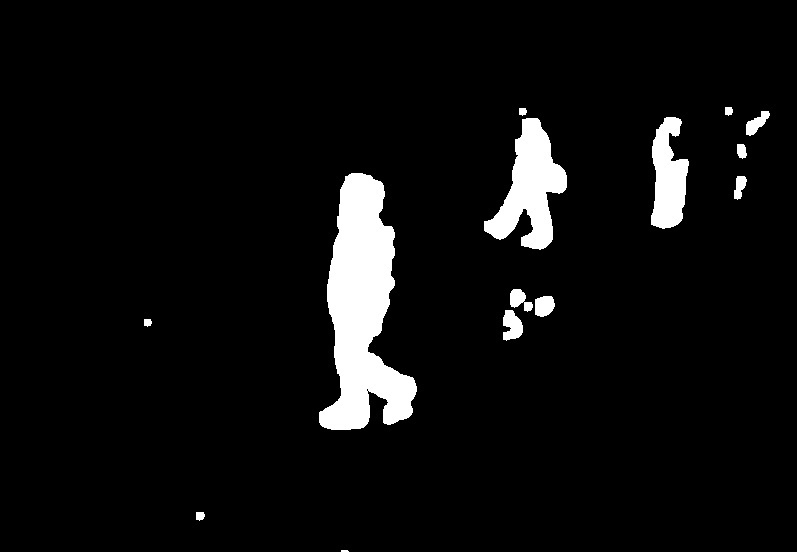
\includegraphics[width=.2\textwidth]{images/mog_original.jpg}\quad
\medskip
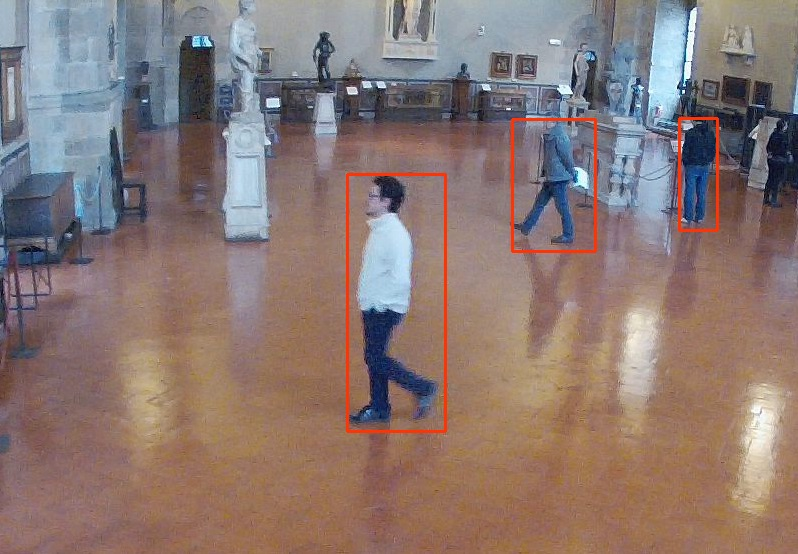
\includegraphics[width=.2\textwidth]{images/motion.jpg}\quad
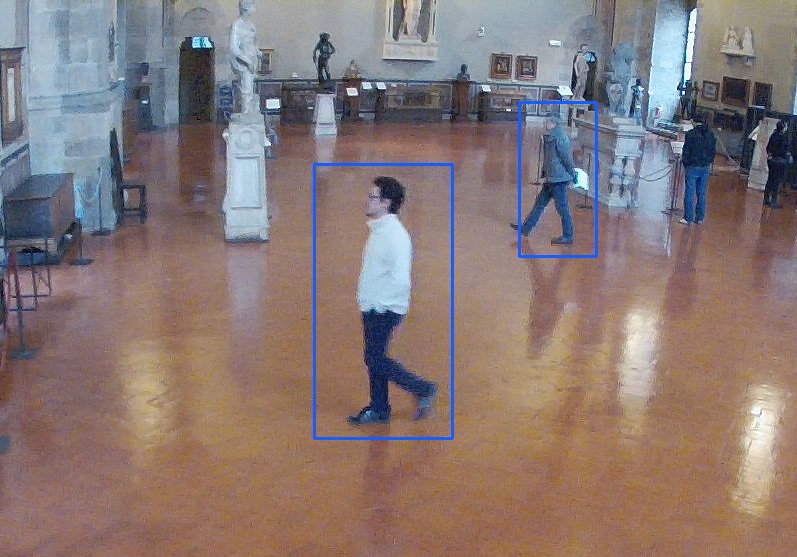
\includegraphics[width=.2\textwidth]{images/pedestrian.jpg}
\caption{Rilevazione oggetti in movimento nella scena tramite \emph{background substraction} (in mezzo) e tramite \emph{pedestrian detection} (in basso). In alto l'immagine originale.}
\label{fig:detections}
\end{figure}

\paragraph{Filtro di Kalman}

Il \emph{filtro di Kalman} è un filtro ricorsivo utilizzato per stimare lo stato successivo di un sistema dinamico a partire da una serie di osservazioni passate che possono essere soggette a rumore. Il filtro è utilizzato in questo elaborato per stimare la posizione successiva del soggetto in caso di assenza di informazioni dagli altri due metodi implementati.

In questo caso il filtro avrà come \emph{stato} le coordinate del centro della bounding box.
Sia $X$ lo \emph{stato del sistema}

\paragraph{La combinazione delle tecniche}

La predizione per ciascuna frame utilizza una combinazione delle tecniche sopra descritte. In base alla bounding box del frame precedente viene intanto selezionata una predizione per ciascuno dei metodi con la condizione che sia parzialmente sovrapposta e compatibile con la previsione passata.

Scartate le bounding box non rilevante, per quelle rimanenti viene calcolato uno \emph{score} definito come:
\begin{equation}
score(r) = \frac{intersection(p, r)}{union(p, r)}
\end{equation}
con $p$ e $r$ rispettivamente la bounding box del frame precedente e la bounding box predetta con una delle due tecniche (motion o pedestrian detection).

A questo punto viene selezionata la predizione con il punteggio più alto ed il filtro di Kalman viene aggiornato con il centro della bounding box selezionata. 

\begin{figure}[h]
\centering
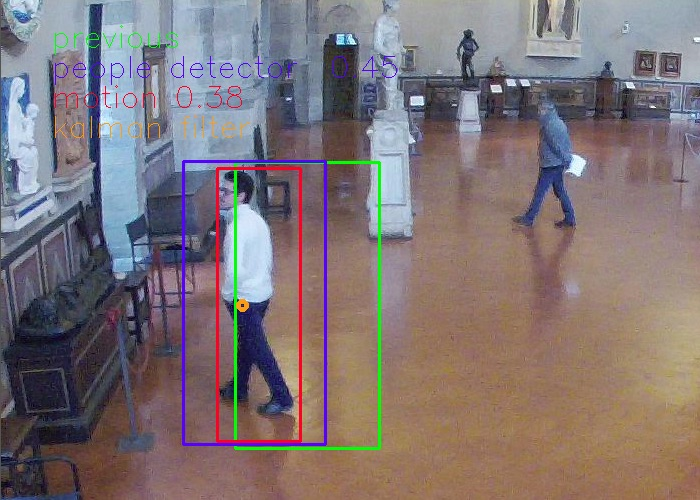
\includegraphics[width=.4\textwidth]{images/prediction1.jpg}\quad
\medskip
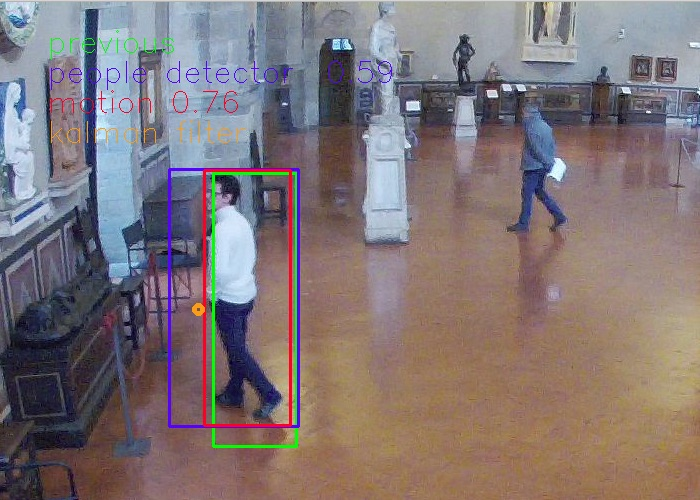
\includegraphics[width=.4\textwidth]{images/prediction2.jpg}\quad
\caption{Esempio di esecuzione dello script con visualizzazione dei risultati parziali su due frame consecutivi. In \emph{verde} la bounding box nella posizione precedente, in \emph{blu} il risultato della pedestrian detection, in \emph{rosso} il risultato del motion detector e in \emph{arancione} il centro predetto tramite filtro di Kalman}
\label{fig:prediction}
\end{figure}

Se non viene rilevata alcuna predizione da motion o pedestrian detection viene considerata valida quella ottenuta tramite filtro di Kalman.


\subsubsection{Geometria della scena}